
Gestures are classified into static gestures and dynamic gestures. Group of static gestures consits of fixed gestures which are not relative to time, where group of dynamic gestures are time varying.

Hand and body gesture recognition had followed a conventional scheme of extracting key features via one or multiple preprocessing sensors and applying machine learning techniques on them.\cite{avola}

The field of gesture recognition gave birth to several image processing devices yielding useful data. One of them being Microsoft Kinect, a device where the main intention was to interpret whole-body movement, making it lacking in required accuracy for hand gesture recognition. 

\section{Leap Motion Controller}
%=======================================================================================================================

Another option would be using a Leap Motion Controller (LMC), developed specifically to track hand movements and extract its features, such as positions of fingers, hand rotation, and others.

LMC consists of two monochromatic IR cameras and three IR LEDs (emitters). 

\begin{figure}[h]
	\centering
    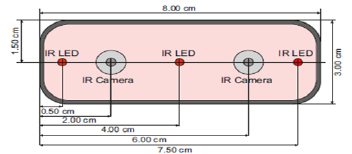
\includegraphics[width=8cm]{lmc_schematic.png}
	\caption{Schematic View of Leap Motion Controller}
	\label{fig:lmcScheme}
\end{figure}



The LMC's current API, Leap Motion Service, yields positions of extracted hand features. All the positional data about the hand and its features are represented in the coordinate system relative to the LMC's center point, positioned at the middle IR LED.\cite{LMCanalysis} The x- and z-axes lie in the camera sensors plane, with the x-axis running along the camera baseline. The y-axis is vertical, with positive values increasing upwards (in contrast to the downward orientation of most computer graphics coordinate systems). The z-axis has positive values increasing toward the user.\cite{tomasMultileap}

\begin{figure}[h]
	\centering
    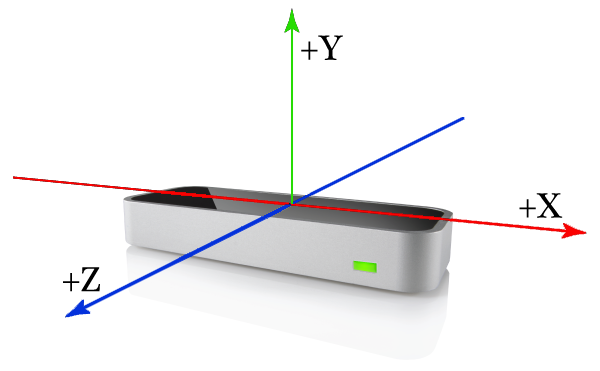
\includegraphics[width=8cm]{leap_axes.png}
	\caption{Leap Motion Controller Axes}
	\label{fig:lmcScheme}
\end{figure}

Unfortunately, Leap Motion Controller has no official library for gesture recognition, limiting developers from utilizing the controller for its key features. Orion, Leap Motion tracking software build for virtual reality, used to have a gesture detector with its 3.0 version, but the detector is absent with the release of more accurate version 4.0.

\section{Methods}
%=======================================================================================================================

Gestures classification should be taken into account when choosing appropriate methods due to their time-varying properties. As previously mentioned, gestures are classified into static and dynamic groups.

\subsection{Static Gesture Recognition}

Common methods for static gesture recognition are Support Vector Machines(SVM), ANN, or pattern techniques.\cite{savaris}.
Mapari and Kharat\cite{mapari} proposed a method to recognize American Sign Language (ASL) by extracting data from LMC and computing 48 features 
(18 positional values, 15 distance values, and 15 angle values) for 4672 collected signs (146 users for 32 signs), eventually feeding them to an ANN using a Multilayer Perceptron (MLP).\cite{katiacnn} Hasan et al.\cite{hasanmlp} proposed a method to recognize six sets of static gestures base on shape analysis using MLP.
Filho et al.\cite{filaml} compared the effectiveness between K-Nearest Neighbors, SVM, and Decision Trees over a dataset of 1200 samples (6 uses for 10 gestures). They normalized positions of the five fingertips and the four angles between adjacent fingers as features to discover that the Decision Tree has performed the best.\cite{katiacnn}

\subsection{Dynamic Gesture Recognition}

\subsection{LSTM}
Many of the proposed methods focus either on static gesture recognition or dynamic gesture recognition, but very few of them are actually utilized for both types at the same time. 